\graphicspath{{images/}}
\section*{Kellerautomaten}

\begin{definition}{Kellerautomaten}
    haben einen «Speicher». PDA = Push Down Automat.\\

    Ein deterministischer Kellerautomat KA ist ein 7-Tupel

    $$
    M=\left(Q, \Sigma, \boldsymbol{\Gamma}, \boldsymbol{\delta}, q_{0}, \$, F\right)
    $$

    \begin{itemize}
    \item Menge von Zuständen: $Q$
    \item Alphabet der Eingabe: $\Sigma$
    \item Alphabet des Kellers: $\Gamma$
    \item Übergangsfunktion: $\boldsymbol{\delta}: \boldsymbol{Q} \times(\boldsymbol{\Sigma} \cup \boldsymbol{\varepsilon}) \times \boldsymbol{\Gamma} \rightarrow \boldsymbol{Q} \times \Gamma^{*}$
    \item Anfangszustand: $q_{0} \in Q$
    \item Symbol vom Alphabet des Kellers: $\$ \in \Gamma$
    \item Akzeptierende Zustände: $F \subseteq Q$
    \end{itemize}
\end{definition}

\begin{concept}{Zusätzliche Einschränkungen für DKAs}\\
    Für jeden Zustand $q$ und alle Symbole $x, b$ gilt, wenn $\delta(q, b, c)$ definiert ist, dann ist $\delta(q, \varepsilon, x)$ undefiniert.

    Ein Übergang $\delta(q, b, c)=(p, \omega)$ wird graphisch dargestellt

    $$
    q -b, c / \omega \longrightarrow p
    $$
\end{concept}

\begin{formula}{Berechnungsschritte}\\
    Ein Berechnungsschritt $\delta(q, b, c)=(p, \omega)$ wird wie folgt interpretiert
    \begin{itemize}
    \item $q=$ Aktueller Zustand
    \item $b=$ Symbol der Eingabe
    \item c = Symbol wird entfernt
    \item $\omega=$ Wort auf Stack geschrieben
    \item $p=$ Neuer Zustand
    \end{itemize}
    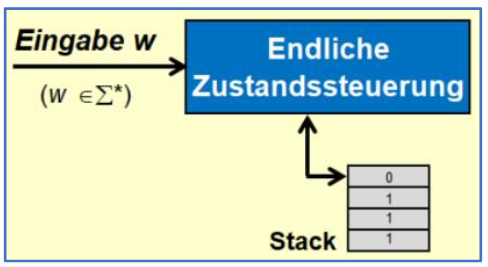
\includegraphics[width=0.3\linewidth]{berechnungsschritte_dka.png}
\end{formula}

\begin{definition}{Sprache eines Kellerautomaten}
    Die Sprache $L(M)$ des Kellerautomaten $M$ ist definiert durch
    $$
    L(M)=\left\{\omega \in \Sigma^{*} \mid\left(q_{0}, \omega, \$\right) \vdash^{*}(q, \varepsilon, \gamma) \text { für ein } q \in F \text { und ein } \gamma \in \Gamma^{*}\right\}
    $$
    Elemente von $L(M)$ werden von $M$ akzeptierte Wörter genannt.
\end{definition}

\begin{KR}{Kellerautomat für eine Sprache erstellen}\\
    Ein Kellerautomat für die kontextfreie Sprache $\left\{0^{n} 1^{n} \mid n>0\right\}$
    \begin{itemize}
    \item $0,0 / 00 \quad$ Read $0 \quad$ Add $0 \quad(00-0)=0$
    \item $0, \$ / 0 \$ \quad$ Read 0 Add $0 \quad(\$ 0-\$)=0$
    \item $1,0 / \varepsilon$ Read 1 Remove 0 Read $(\varepsilon-0)=-0$
    \item $\varepsilon, \$ / \$ \quad$ Read $\varepsilon$ - $(\$-\$)=\varepsilon$
    \end{itemize}
    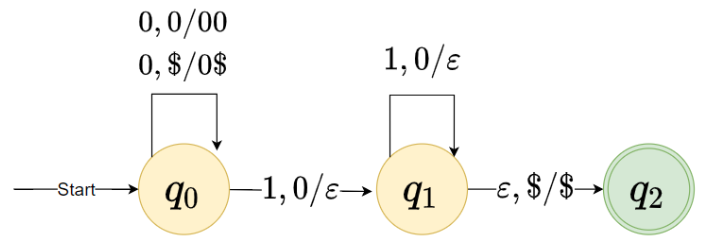
\includegraphics[width=0.3\linewidth]{kellerautomat_sprache.png}
    \begin{itemize}
        \item $\omega_{1}=011:\left(q_{0}, 011, \$\right) \vdash\left(q_{1}, 11,0 \$\right) \vdash\left(q_{1}, 1, \$\right) \rightarrow \omega_{1}$ verwerfend
    \end{itemize}
    Das Zeichen \$ zeigt an, dass der «Stack» leer ist.
\end{KR}

\begin{concept}{NKA: Übergangsfunktion}
    \begin{itemize}
        \item $\delta: Q \times(\Sigma \cup \varepsilon) \times \Gamma \rightarrow P(Q \times \Gamma *)$
    \end{itemize}
    Kellerautomat für die Sprache $\left\{\omega \omega^{R} \mid \omega \in\{0,1\}^{*}\right\}$\\
    \includegraphics[width=0.3\linewidth]{nka_übergangsfunktion.png}
\end{concept}